\documentclass[a4paper,12pt]{article}
\usepackage{fullpage}
\usepackage[utf8x]{inputenc}
\usepackage{fancyhdr}
\usepackage{booktabs}
\usepackage[hang,bf,small]{caption}
\usepackage{color}
\usepackage{graphicx}
\usepackage{multirow}
\usepackage{hyperref}
\usepackage{longtable}
\usepackage{subfig}


%set subfig package options
\captionsetup[subfloat]{position=top,singlelinecheck=false,labelfont={normalsize,sf},
labelformat=simple,listofformat=subparens,aboveskip=0pt,parskip=0pt,farskip=0pt,captionskip=0pt}

%customize subfigure label to capitals
\renewcommand{\thesubfigure}{\Alph{subfigure}}
\renewcommand{\thesubtable}{\textbf{\Alph{subtable}}}



\begin{document}

\begin{titlepage}

\begin{center}

\textsc{ }\\[2cm]
% Upper part of the page
%\includegraphics[width=0.7\textwidth]{img/logoTRANSPAT.jpg}\\[4cm]    


\textsc{\textcolor{blue}{\Huge \em Integrated Gene Set Analysis for microRNA Studies}}\\[2.5cm]


\textsc{\textcolor{blue}{\Large Exploratory Analysis for Enrichment Results}}\\[2.5cm]


%\includegraphics[width=0.3\textwidth]{img/logoERANET.jpg}\\[4cm]    


% Title
% \HRule \\[0.4cm]
% { \Large Computational Genomics Department}\\[0.4cm]
% { \Large CIPF, Valencia (Spain)}\\[0.4cm]



\vfill

% Bottom of the page
{\large \today}

\end{center}

\end{titlepage}


% \maketitle

\tableofcontents


% \begin{abstract}
% \end{abstract}
\cleardoublepage




\section{Overview}\label{secOverview}

The goal is to detect similar cancer groups from functional enrichment results. We generate an indicator for each GO term:  sign (log(OR)) * -1 * log(raw pvalue) from \textbf{mdgsa} 
(\url{http://www.bioconductor.org/packages/release/bioc/html/mdgsa.html}). 
We perform clustering and principal components analysis to explore relationships between groups of tumors. 




\begin{figure}[!h] 
\centering 
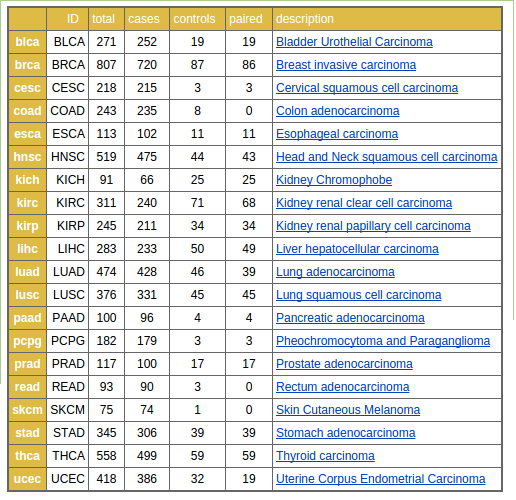
\includegraphics[width=0.6\textwidth]{img/table1.png} 
\caption{Analyzed datasets. Columns on the table display: TCGA disease ID, the total number of samples in the  analysis, the 
 number of tumoral samples, the number  of control samples  (solid  normal tissue), the number of paired samples available in the 
 dataset and the cancer type} 
\label{figDESCRIPTION} 
\end{figure} 

\clearpage



\section{Principal Component Analysis}

The PCA plots below show the first three principal components of all samples in the study. 
See \url{http://en.wikipedia.org/wiki/Principal_component_analysis} for details on Principal Component Analysis.

\begin{figure}[!h] 
\centering 
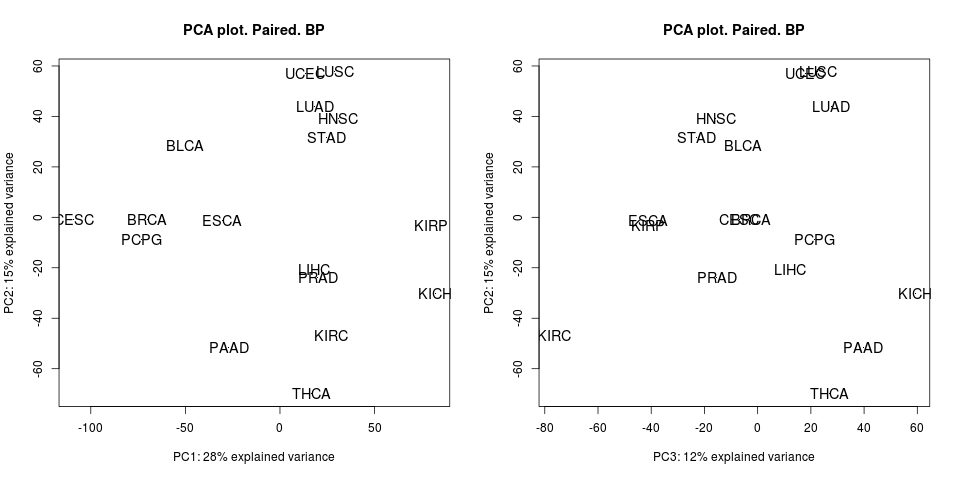
\includegraphics[width=0.9\textwidth]{img/pca_bp_paired.png} 
\caption{PCAplot from enrichment results (Biological Processes) in TCGA paired studies} 
\label{figPCA_bp_paired} 
\end{figure} 

\begin{figure}[!h] 
\centering 
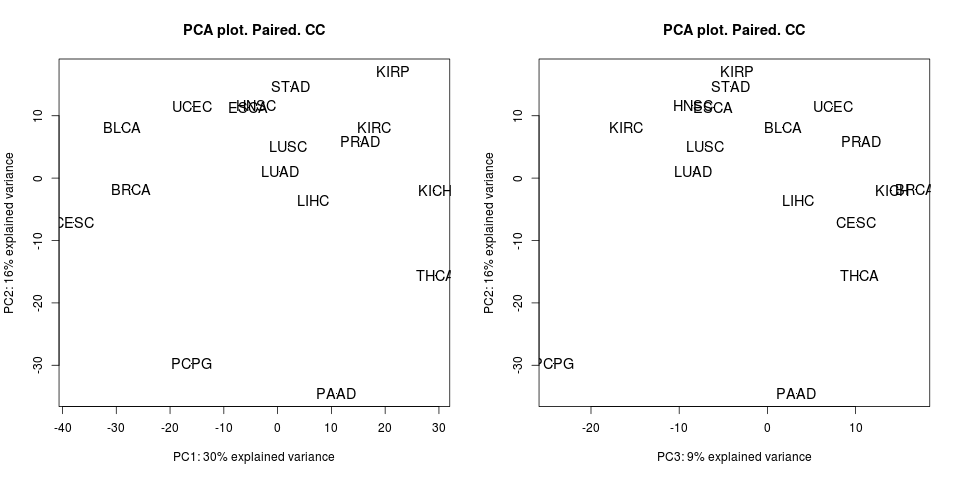
\includegraphics[width=0.9\textwidth]{img/pca_cc_paired.png} 
\caption{PCAplot from enrichment results (Cellular Components) in TCGA paired studies} 
\label{figPCA_cc_paired} 
\end{figure} 

\begin{figure}[!h] 
\centering 
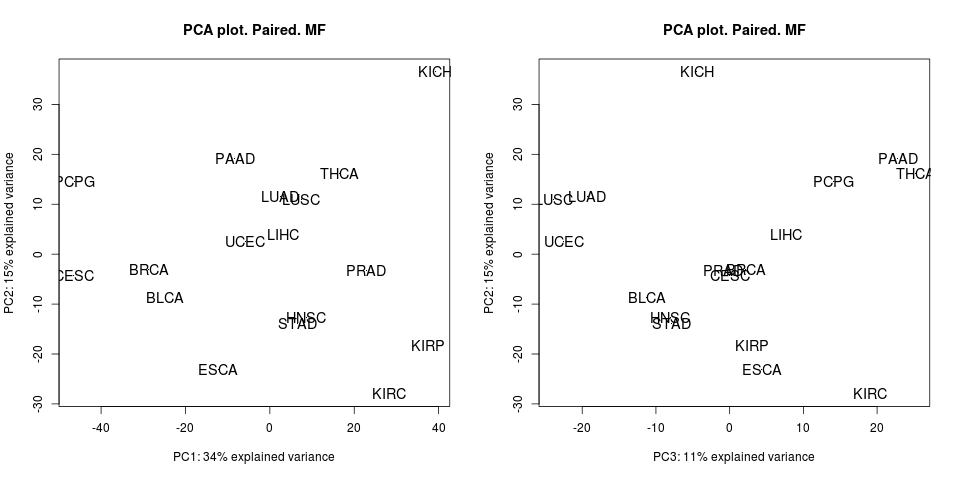
\includegraphics[width=0.9\textwidth]{img/pca_mf_paired.png} 
\caption{PCAplot from enrichment results (Molecular Functions) in TCGA paired studies} 
\label{figPCA_mf_paired} 
\end{figure} 


\begin{figure}[!h] 
\centering 
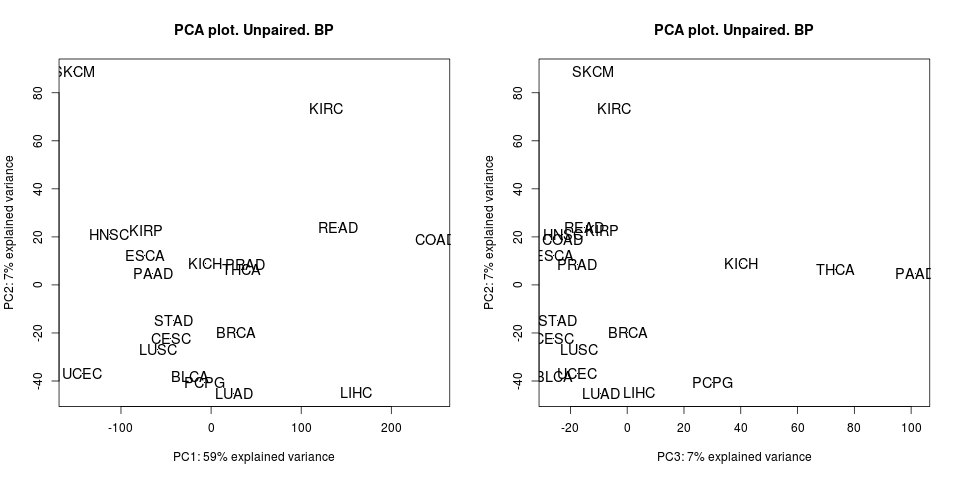
\includegraphics[width=0.9\textwidth]{img/pca_bp_unpaired.png} 
\caption{PCAplot from enrichment results (Biological Processes) in TCGA unpaired studies} 
\label{figPCA_bp_unpaired} 
\end{figure} 

\begin{figure}[!h] 
\centering 
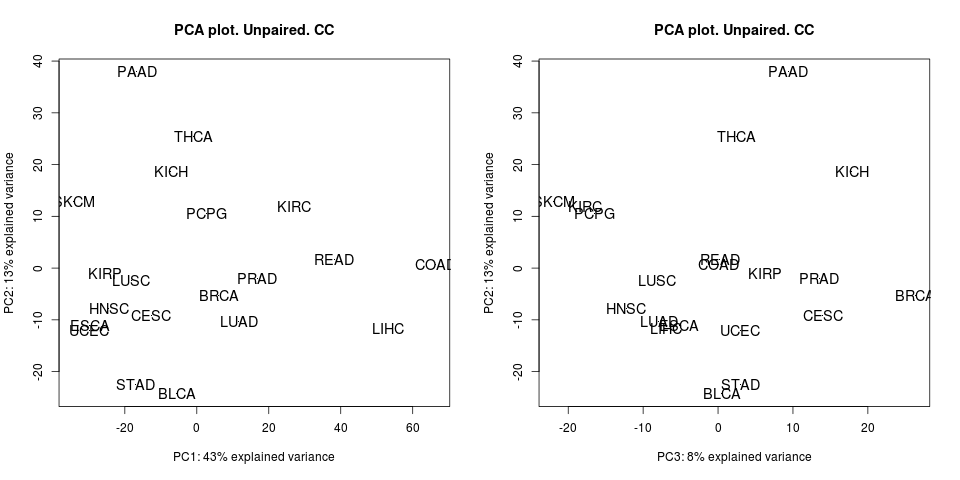
\includegraphics[width=0.9\textwidth]{img/pca_cc_unpaired.png} 
\caption{PCAplot from enrichment results (Cellular Components) in TCGA unpaired studies} 
\label{figPCA_cc_unpaired} 
\end{figure} 

\begin{figure}[!h] 
\centering 
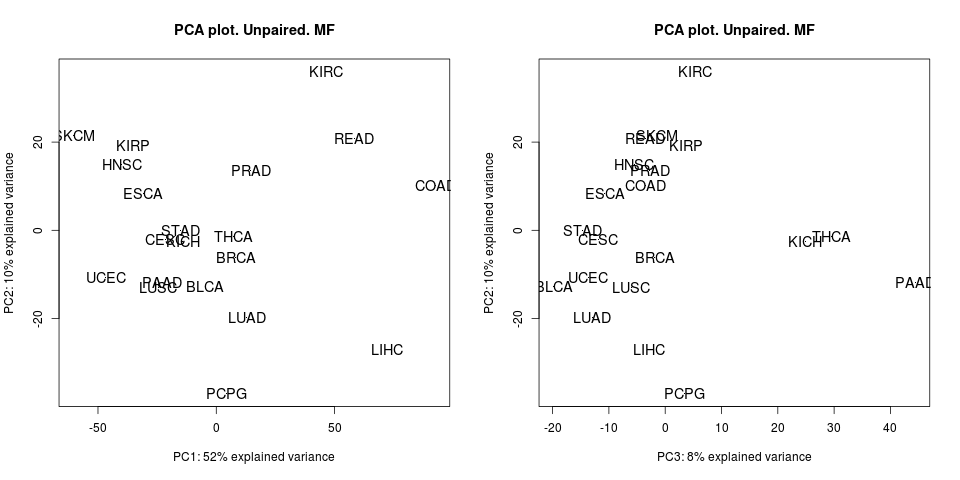
\includegraphics[width=0.9\textwidth]{img/pca_mf_unpaired.png} 
\caption{PCAplot from enrichment results (Molecular Functions) in TCGA unpaired studies} 
\label{figPCA_mf_unpaired} 
\end{figure} 

\clearpage

\section{Clustering Analysis}

Complete linkage method was used for hierarchical clustering. 
This particular clustering method defines the cluster distance between two clusters to be the maximum distance between their individual components.
At every stage of the clustering process, the two nearest clusters are merged into a new cluster. 
The process is repeated until the whole data set is agglomerated into one single cluster. Two distances were used: euclidean and Pearson correlation.


\subsection{Clustering Analysis, euclidean distance}
\begin{figure}[!h] 
\centering 
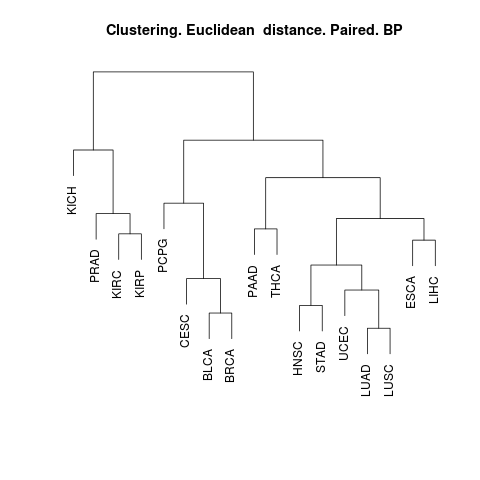
\includegraphics[width=0.6\textwidth]{img/cluster_euclideand_bp_paired.png} 
\caption{Clustering from enrichment results (Biological Processes), euclidean distance.  TCGA paired studies} 
\label{figCLUST_eu_bp_paired} 
\end{figure} 

\begin{figure}[!h] 
\centering 
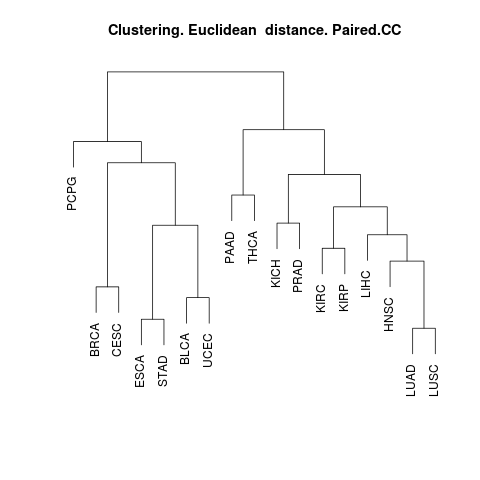
\includegraphics[width=0.6\textwidth]{img/cluster_euclideand_cc_paired.png} 
\caption{Clustering from enrichment results (Cellular Components), euclidean distance.  TCGA paired studies} 
\label{figCLUST_eu_cc_paired} 
\end{figure} 

\begin{figure}[!h] 
\centering 
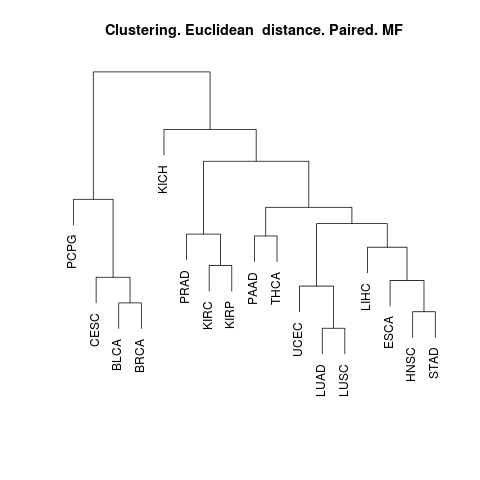
\includegraphics[width=0.6\textwidth]{img/cluster_euclideand_mf_paired.png} 
\caption{Clustering from enrichment results (Molecular Functions), euclidean distance.  TCGA paired studies} 
\label{figCLUST_eu_mf_paired} 
\end{figure} 



\begin{figure}[!h] 
\centering 
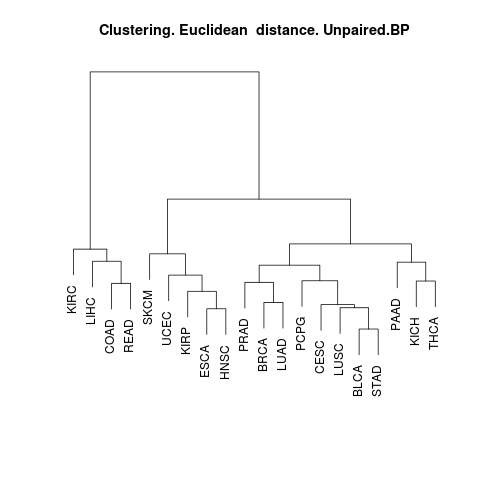
\includegraphics[width=0.6\textwidth]{img/cluster_euclideand_bp_unpaired.png} 
\caption{Clustering from enrichment results (Biological Processes), euclidean distance.  TCGA unpaired studies} 
\label{figCLUST_eu_bp_unpaired} 
\end{figure} 

\begin{figure}[!h] 
\centering 
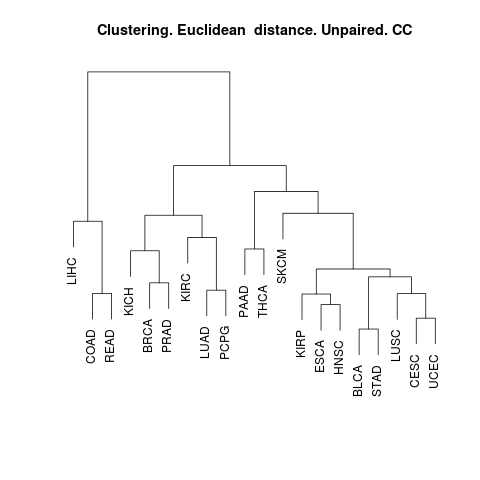
\includegraphics[width=0.6\textwidth]{img/cluster_euclideand_cc_unpaired.png} 
\caption{Clustering from enrichment results (Cellular Components), euclidean distance.  TCGA unpaired studies} 
\label{figCLUST_eu_cc_unpaired} 
\end{figure} 

\begin{figure}[!h] 
\centering 
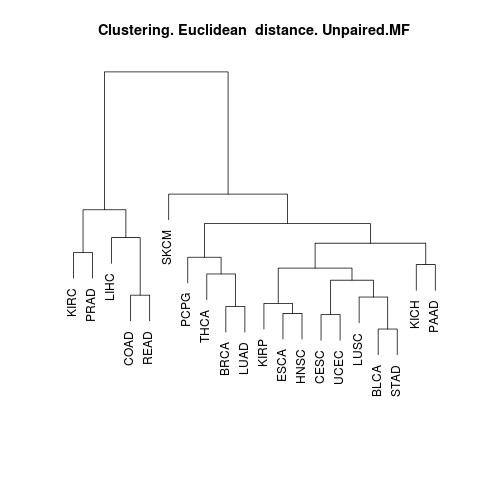
\includegraphics[width=0.6\textwidth]{img/cluster_euclideand_mf_unpaired.png} 
\caption{Clustering from enrichment results (Molecular Functions), euclidean distance.  TCGA unpaired studies} 
\label{figCLUST_eu_mf_unpaired} 
\end{figure} 
\clearpage


\subsection{Clustering Analysis, correlation distance}

\begin{figure}[!h] 
\centering 
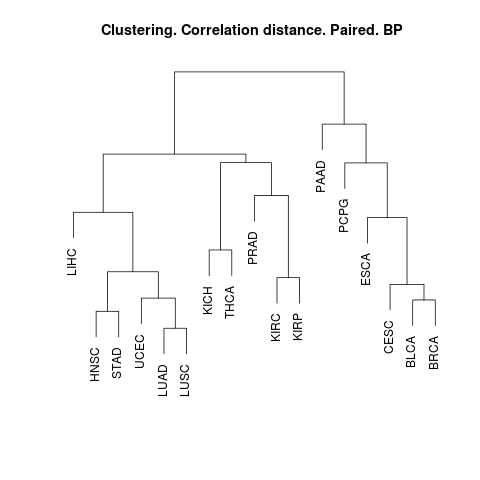
\includegraphics[width=0.6\textwidth]{img/cluster_corelationd_bp_paired.png} 
\caption{Clustering from enrichment results (Biological Processes), correlation distance.  TCGA paired studies} 
\label{figCLUST_corr_bp_paired} 
\end{figure} 

\begin{figure}[!h] 
\centering 
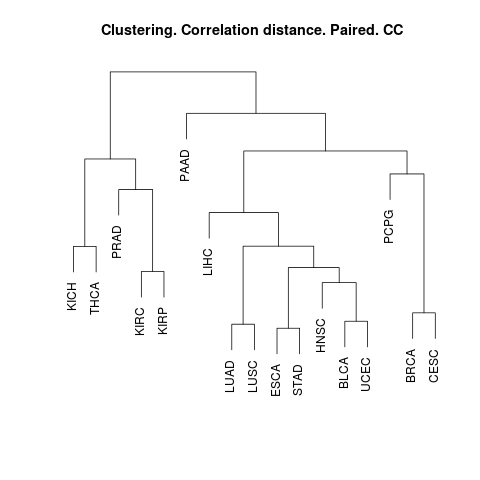
\includegraphics[width=0.6\textwidth]{img/cluster_corelationd_cc_paired.png} 
\caption{Clustering from enrichment results (Cellular Components), correlation distance.  TCGA paired studies} 
\label{figCLUST_corr_cc_paired} 
\end{figure} 

\begin{figure}[!h] 
\centering 
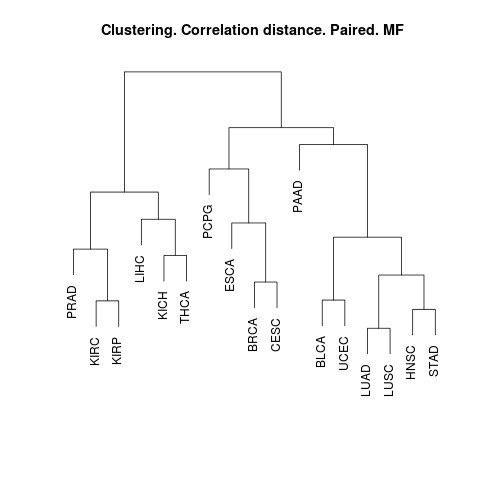
\includegraphics[width=0.6\textwidth]{img/cluster_corelationd_mf_paired.png} 
\caption{Clustering from enrichment results (Molecular Functions), correlation distance.  TCGA paired studies} 
\label{figCLUST_corr_mf_paired} 
\end{figure} 



\begin{figure}[!h] 
\centering 
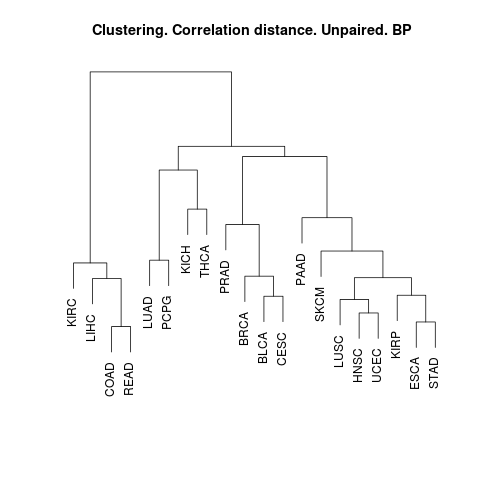
\includegraphics[width=0.6\textwidth]{img/cluster_corelationd_bp_unpaired.png} 
\caption{Clustering from enrichment results (Biological Processes), correlation distance.  TCGA unpaired studies} 
\label{figCLUST_corr_bp_unpaired} 
\end{figure} 

\begin{figure}[!h] 
\centering 
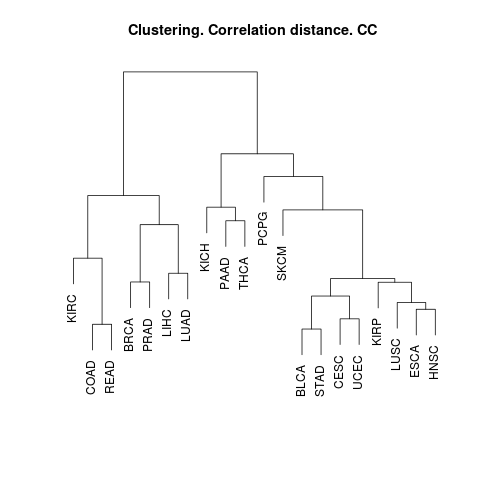
\includegraphics[width=0.6\textwidth]{img/cluster_corelationd_cc_unpaired.png} 
\caption{Clustering from enrichment results (Cellular Components), correlation distance.  TCGA unpaired studies} 
\label{figCLUST_corr_cc_unpaired} 
\end{figure} 

\begin{figure}[!h] 
\centering 
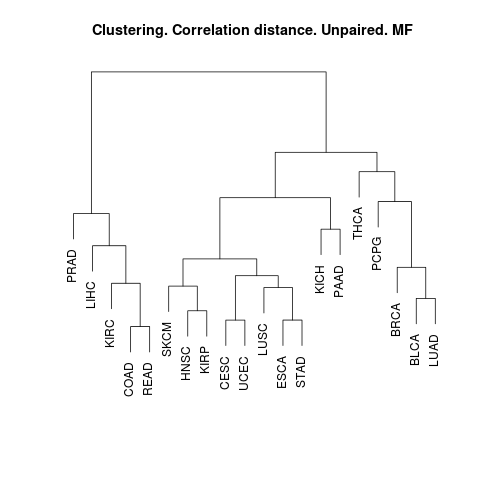
\includegraphics[width=0.6\textwidth]{img/cluster_corelationd_mf_unpaired.png} 
\caption{Clustering from enrichment results (Molecular Functions), correlation distance.  TCGA unpaired studies} 
\label{figCLUST_corr_mf_unpaired} 
\end{figure} 
\clearpage

\subsection{Significant Clustering Analysis, correlation distance}
Cluster analysis was evaluated from \textbf{pvclust} (\url{http://www.sigmath.es.osaka-u.ac.jp/shimo-lab/prog/pvclust/}). 
This R package calculates probability values (p-values) for each cluster using bootstrap resampling techniques.

P-value of a cluster is a value between 0 and 1, which indicates how strong the cluster is supported by data.
\textbf{pvclust} provides two types of p-values: AU (Approximately Unbiased) p-value and BP (Bootstrap Probability) value. 
AU p-value, which is computed by multiscale bootstrap resampling, is a better approximation to unbiased p-value than BP value 
computed by normal bootstrap resampling.

\textbf{pvclust} performs hierarchical cluster analysis via function hclust and automatically computes p-values 
for all clusters contained in the clustering of original data. It also provides graphical tools such as plot function 
or useful pvrect function which highlights clusters with relatively high/low p-values. 





\begin{figure}[!h] 
\centering 
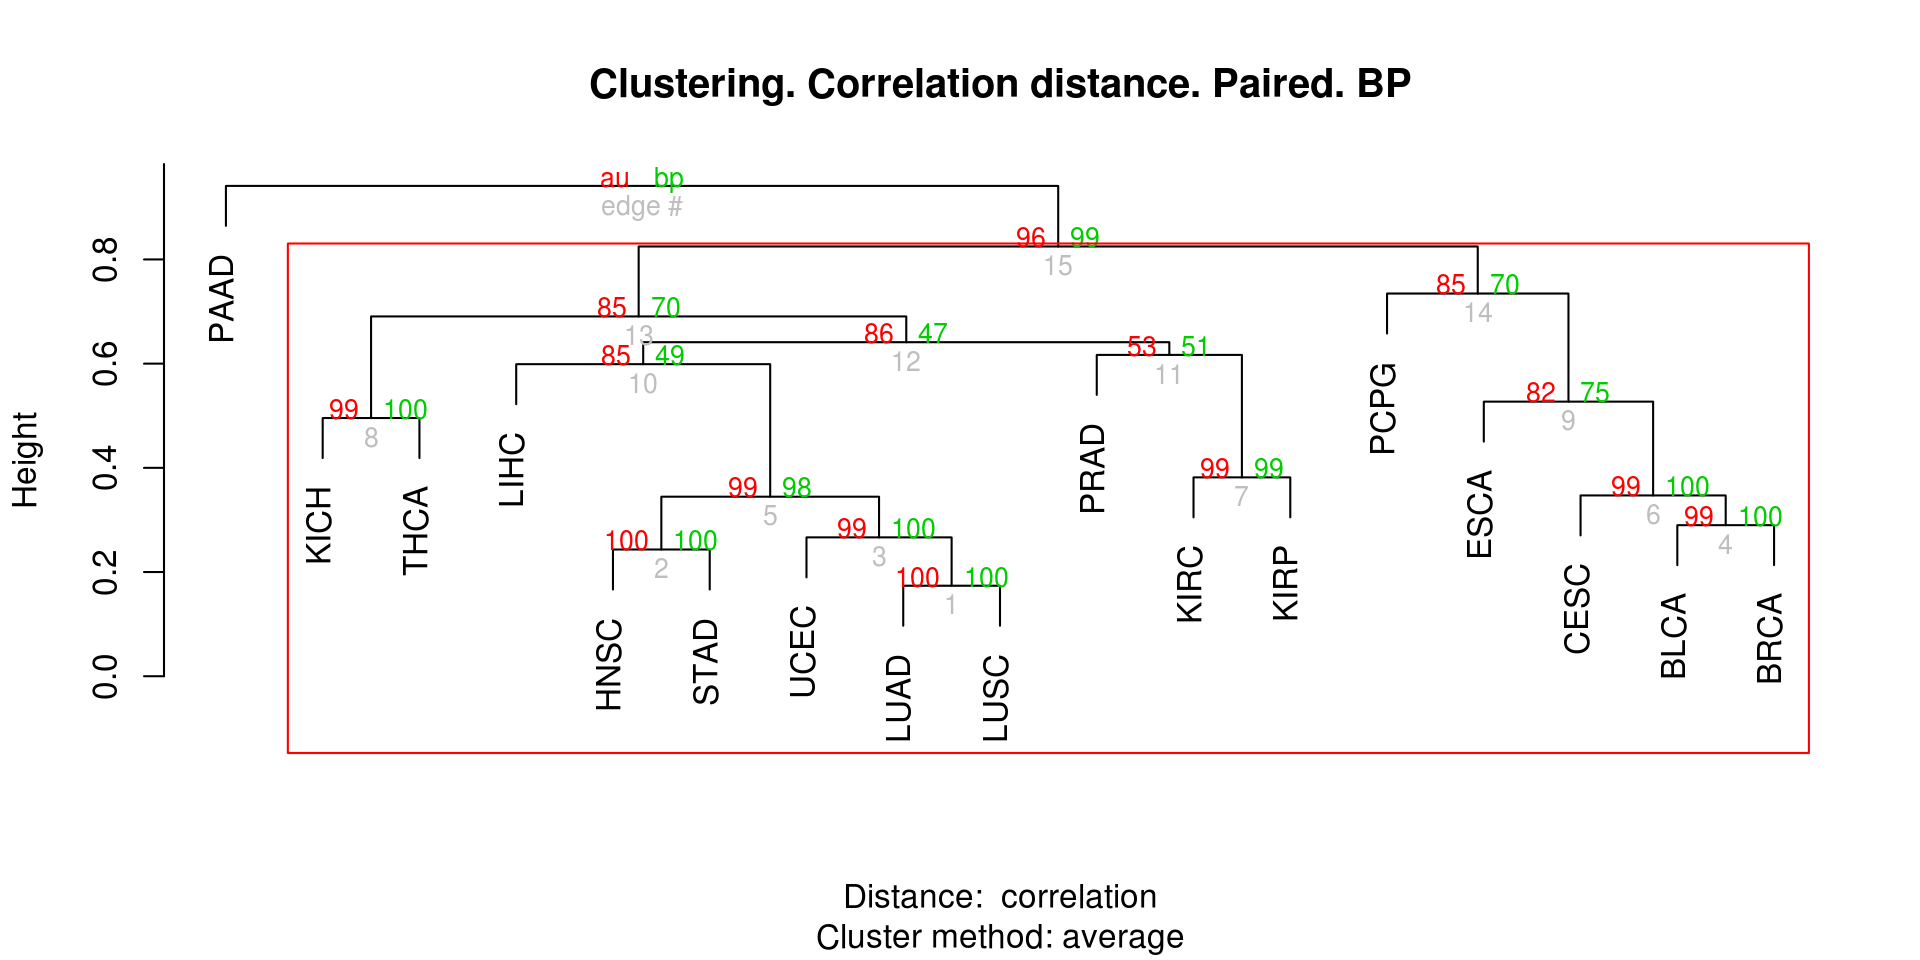
\includegraphics[width=1\textwidth]{img/sigcluster_corelationd_bp_paired.png} 
\caption{Significant clustering from enrichment results (Biological Processes), correlation distance.  TCGA paired studies} 
\label{figCLUSTsig_corr_bp_paired} 
\end{figure} 

\begin{figure}[!h] 
\centering 
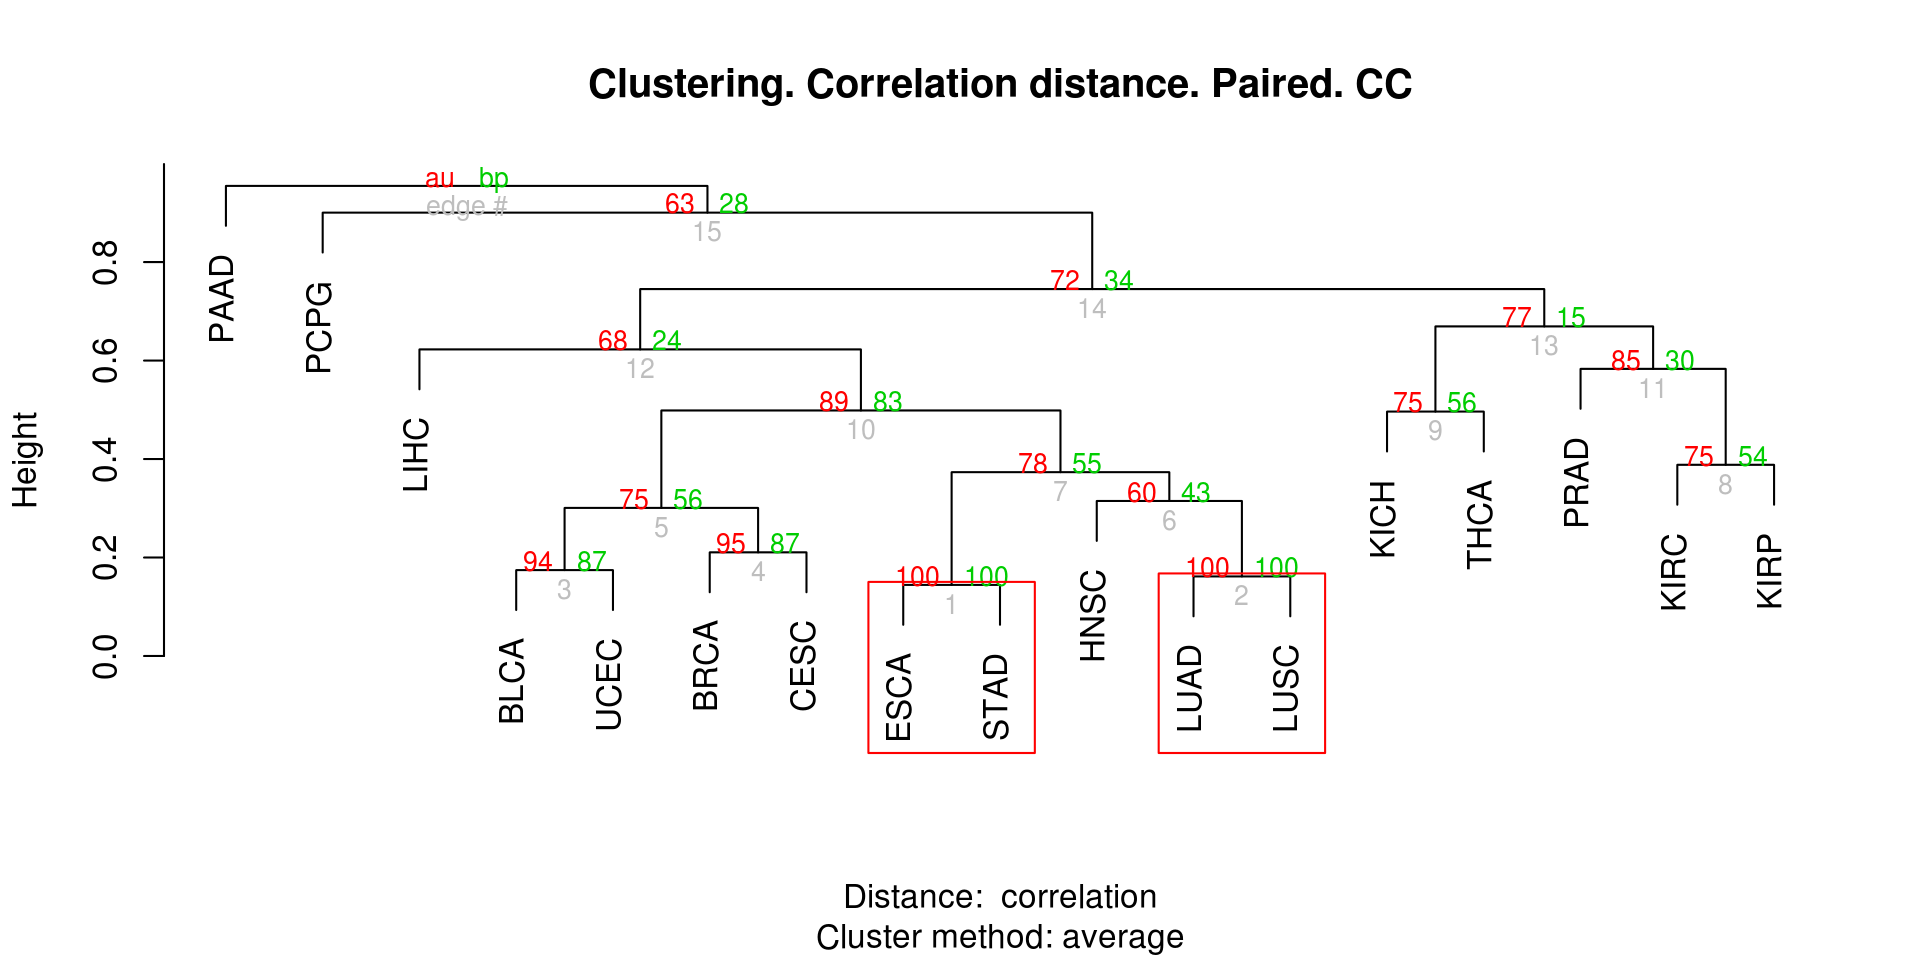
\includegraphics[width=1\textwidth]{img/sigcluster_corelationd_cc_paired.png} 
\caption{Significant clustering from enrichment results (Cellular Components), correlation distance.  TCGA paired studies} 
\label{figCLUSTsig_corr_cc_paired} 
\end{figure} 

\begin{figure}[!h] 
\centering 
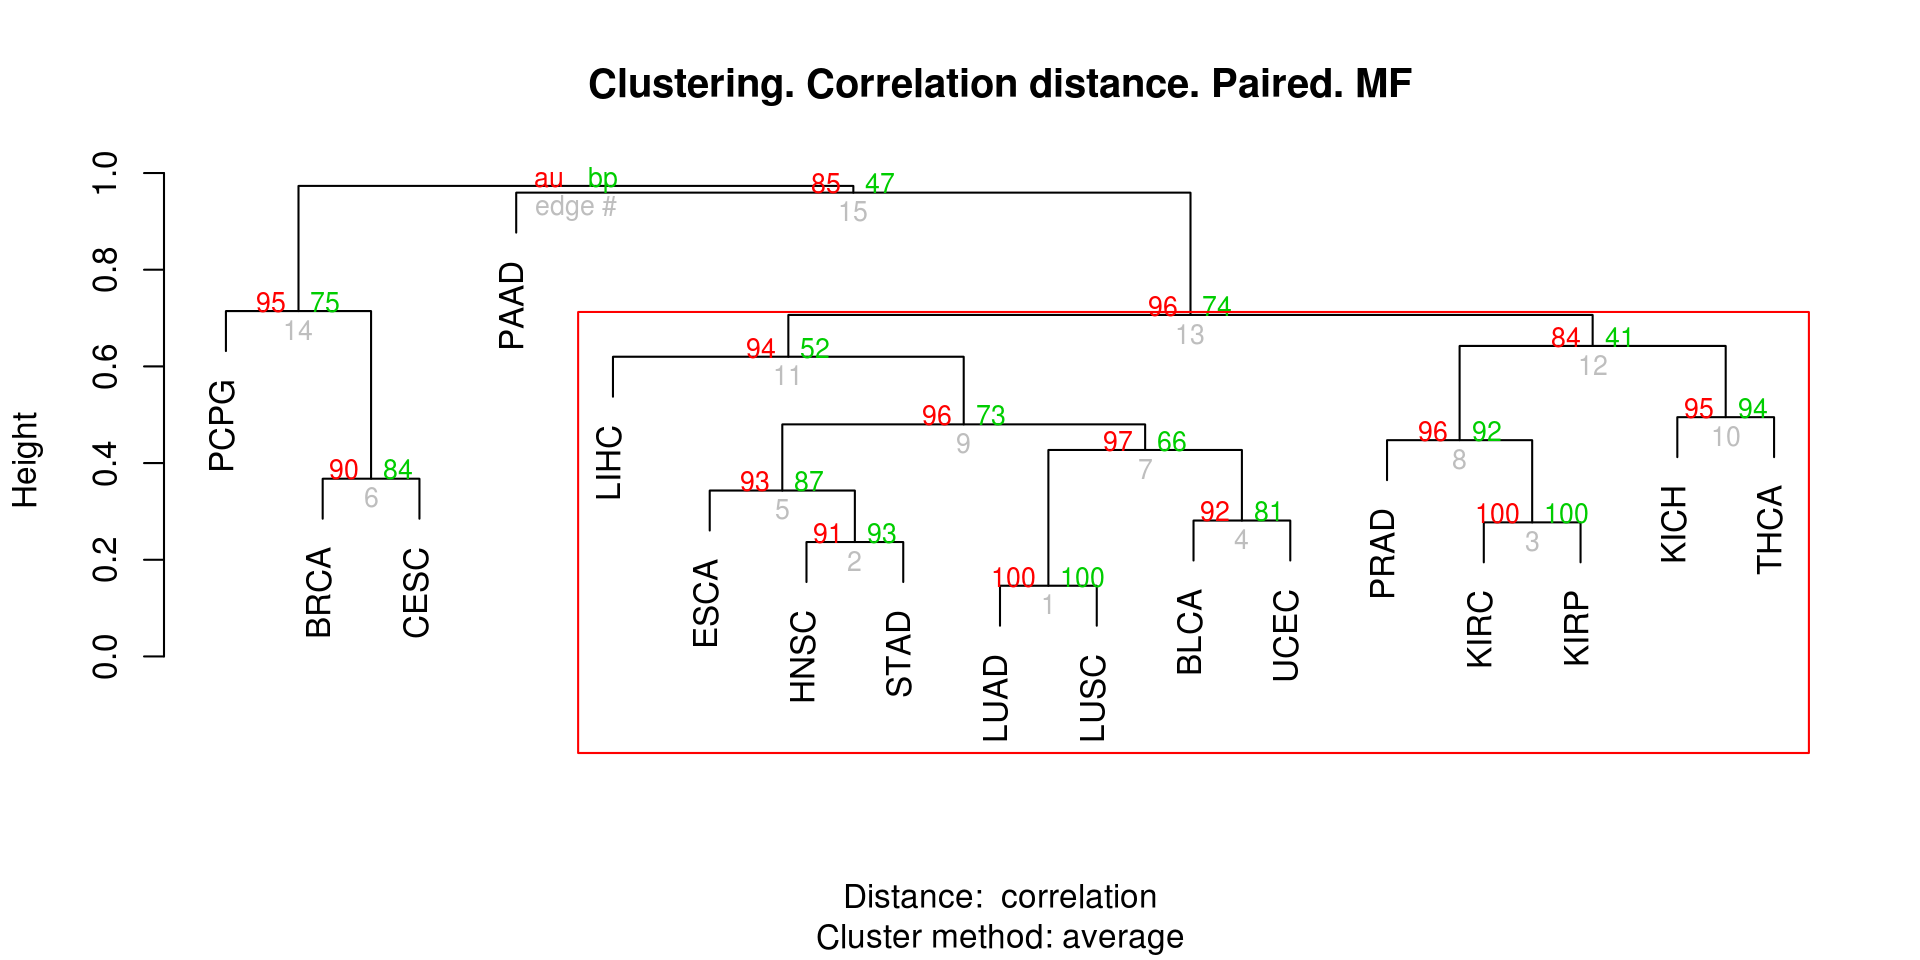
\includegraphics[width=1\textwidth]{img/sigcluster_corelationd_mf_paired.png} 
\caption{Significant clustering from enrichment results (Molecular Functions), correlation distance.  TCGA paired studies} 
\label{figCLUSTsig_corr_mf_paired} 
\end{figure} 



\begin{figure}[!h] 
\centering 
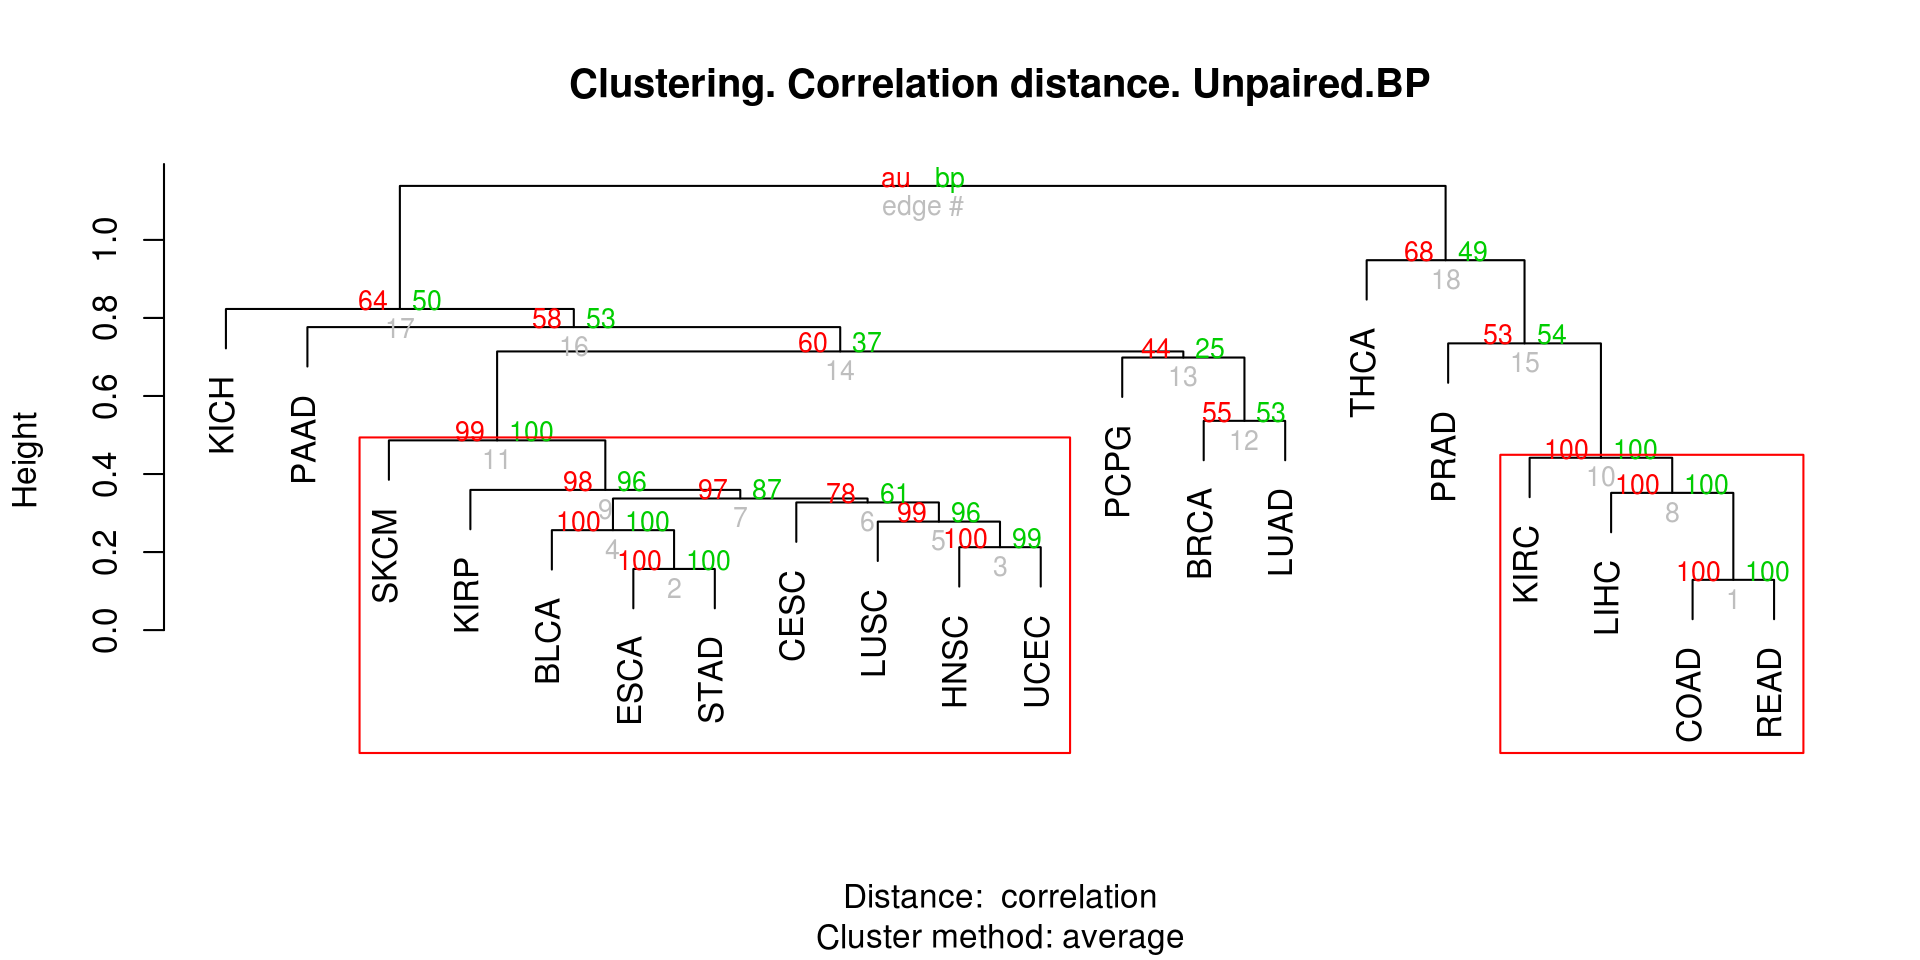
\includegraphics[width=1\textwidth]{img/sigcluster_corelationd_bp_unpaired.png} 
\caption{Significant clustering from enrichment results (Biological Processes), correlation distance.  TCGA unpaired studies} 
\label{figCLUSTsig_corr_bp_unpaired} 
\end{figure} 

\begin{figure}[!h] 
\centering 
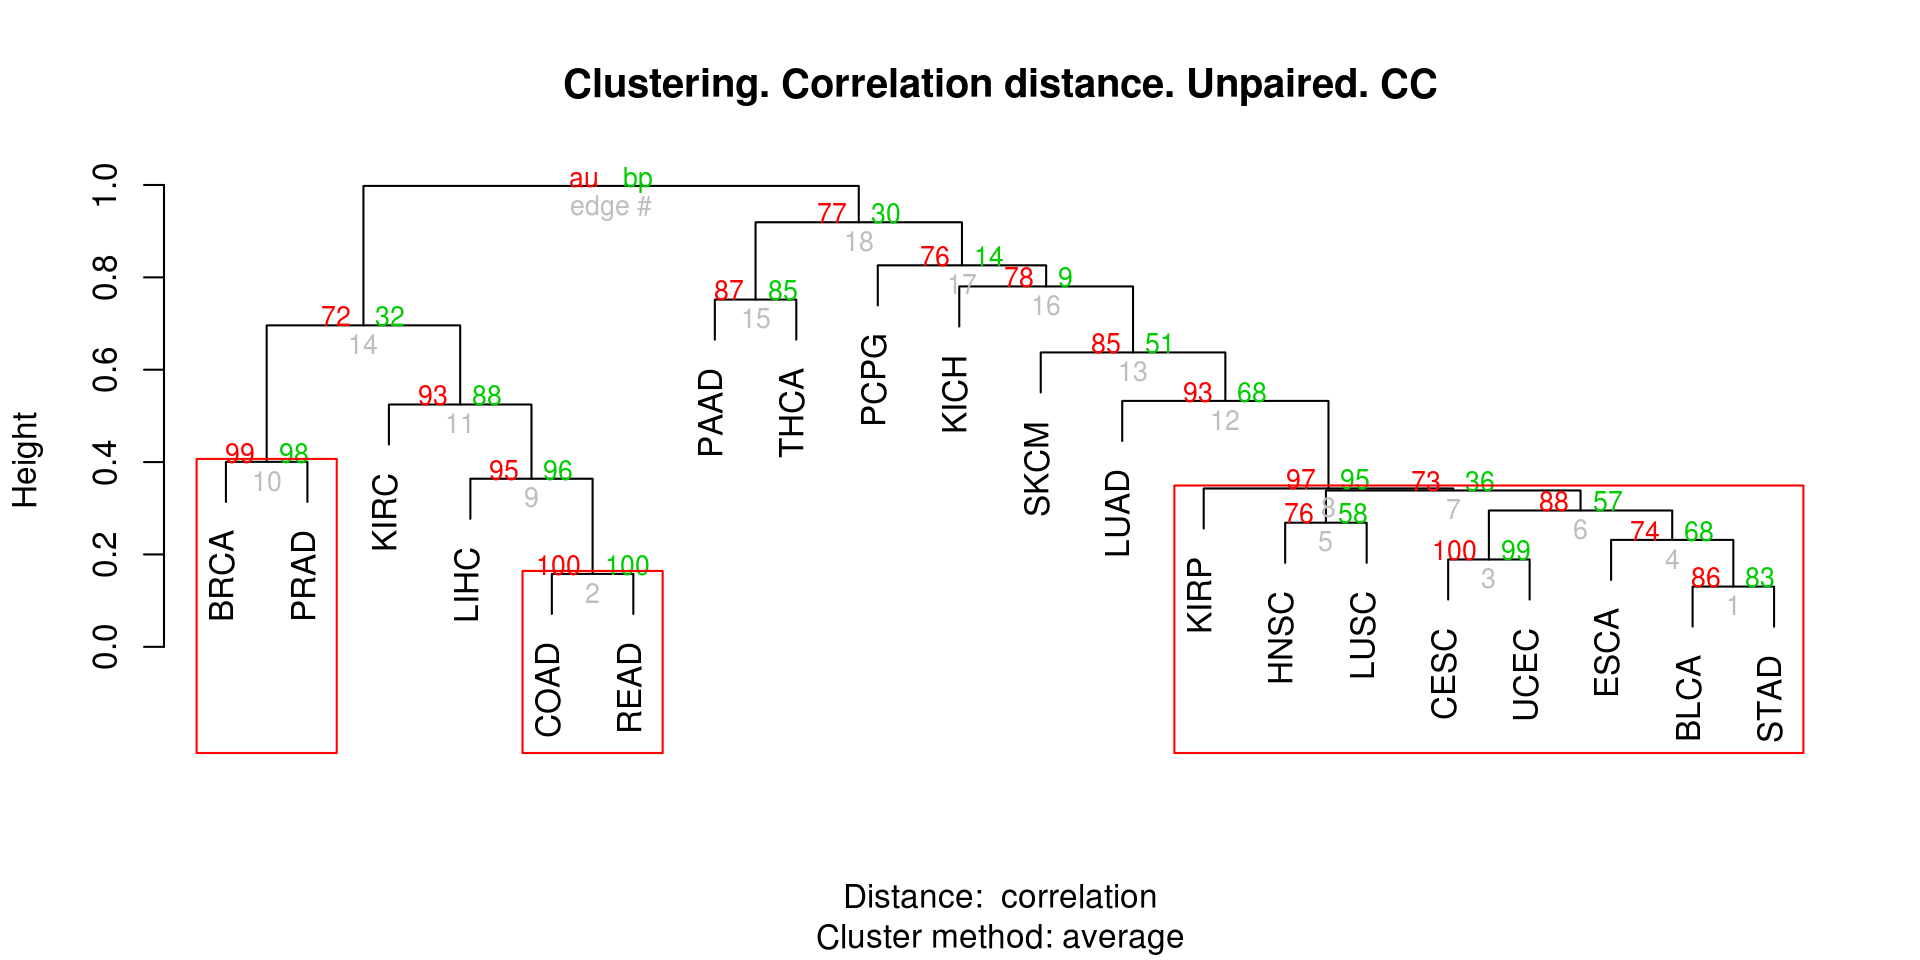
\includegraphics[width=1\textwidth]{img/sigcluster_corelationd_cc_unpaired.png} 
\caption{Significant clustering from enrichment results (Cellular Components), correlation distance.  TCGA unpaired studies} 
\label{figCLUSTsig_corr_cc_unpaired} 
\end{figure} 

\begin{figure}[!h] 
\centering 
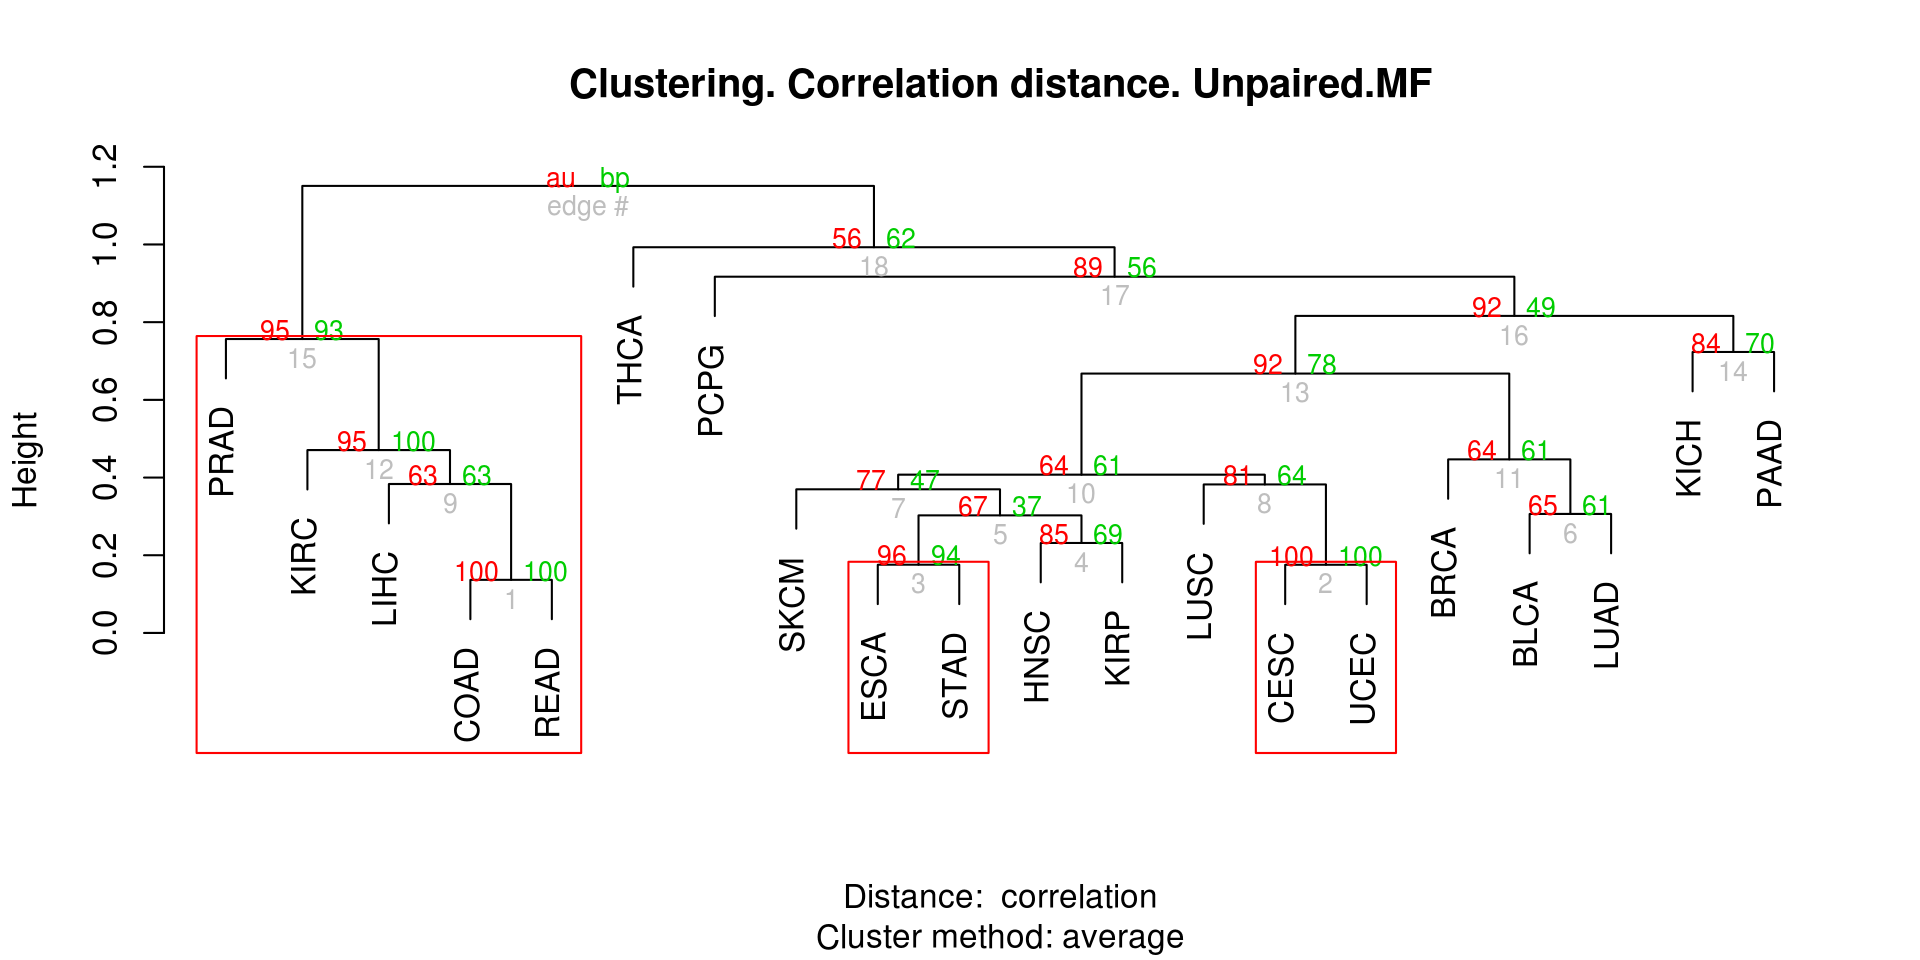
\includegraphics[width=1\textwidth]{img/sigcluster_corelationd_mf_unpaired.png} 
\caption{Significant clustering from enrichment results (Molecular Functions), correlation distance.  TCGA unpaired studies} 
\label{figCLUSTsig_corr_mf_unpaired} 
\end{figure} 
\clearpage








\addcontentsline{toc}{section}{References}
% \addcontentsline{toc}{chapter}{\numberline{}\bibname}


\bibliographystyle{abbrv}
\bibliography{clustering}
\begin{itemize}
 \item Everitt, B. (1974). Cluster Analysis. London: Heinemann Educ. Books.
 \item Suzuki R and Shimodaira H (2006).  Pvclust: an R package for assessing the uncertainty in hierarchical clustering. Bioinformatics. Jun 15;22(12):1540-2. Epub 2006 Apr 4.
 \item Montaner D and Dopazo J (2010). Multidimensional Gene Set Analysis of Genomic Data. PLoS One, 5(4), pp. e10348. 
\end{itemize}







\end{document}   